% Options for packages loaded elsewhere
\PassOptionsToPackage{unicode}{hyperref}
\PassOptionsToPackage{hyphens}{url}
%
\documentclass[
]{article}
\usepackage{amsmath,amssymb}
\usepackage{iftex}
\ifPDFTeX
  \usepackage[T1]{fontenc}
  \usepackage[utf8]{inputenc}
  \usepackage{textcomp} % provide euro and other symbols
\else % if luatex or xetex
  \usepackage{unicode-math} % this also loads fontspec
  \defaultfontfeatures{Scale=MatchLowercase}
  \defaultfontfeatures[\rmfamily]{Ligatures=TeX,Scale=1}
\fi
\usepackage{lmodern}
\ifPDFTeX\else
  % xetex/luatex font selection
\fi
% Use upquote if available, for straight quotes in verbatim environments
\IfFileExists{upquote.sty}{\usepackage{upquote}}{}
\IfFileExists{microtype.sty}{% use microtype if available
  \usepackage[]{microtype}
  \UseMicrotypeSet[protrusion]{basicmath} % disable protrusion for tt fonts
}{}
\makeatletter
\@ifundefined{KOMAClassName}{% if non-KOMA class
  \IfFileExists{parskip.sty}{%
    \usepackage{parskip}
  }{% else
    \setlength{\parindent}{0pt}
    \setlength{\parskip}{6pt plus 2pt minus 1pt}}
}{% if KOMA class
  \KOMAoptions{parskip=half}}
\makeatother
\usepackage{xcolor}
\usepackage[margin=2.54cm]{geometry}
\usepackage{color}
\usepackage{fancyvrb}
\newcommand{\VerbBar}{|}
\newcommand{\VERB}{\Verb[commandchars=\\\{\}]}
\DefineVerbatimEnvironment{Highlighting}{Verbatim}{commandchars=\\\{\}}
% Add ',fontsize=\small' for more characters per line
\usepackage{framed}
\definecolor{shadecolor}{RGB}{248,248,248}
\newenvironment{Shaded}{\begin{snugshade}}{\end{snugshade}}
\newcommand{\AlertTok}[1]{\textcolor[rgb]{0.94,0.16,0.16}{#1}}
\newcommand{\AnnotationTok}[1]{\textcolor[rgb]{0.56,0.35,0.01}{\textbf{\textit{#1}}}}
\newcommand{\AttributeTok}[1]{\textcolor[rgb]{0.13,0.29,0.53}{#1}}
\newcommand{\BaseNTok}[1]{\textcolor[rgb]{0.00,0.00,0.81}{#1}}
\newcommand{\BuiltInTok}[1]{#1}
\newcommand{\CharTok}[1]{\textcolor[rgb]{0.31,0.60,0.02}{#1}}
\newcommand{\CommentTok}[1]{\textcolor[rgb]{0.56,0.35,0.01}{\textit{#1}}}
\newcommand{\CommentVarTok}[1]{\textcolor[rgb]{0.56,0.35,0.01}{\textbf{\textit{#1}}}}
\newcommand{\ConstantTok}[1]{\textcolor[rgb]{0.56,0.35,0.01}{#1}}
\newcommand{\ControlFlowTok}[1]{\textcolor[rgb]{0.13,0.29,0.53}{\textbf{#1}}}
\newcommand{\DataTypeTok}[1]{\textcolor[rgb]{0.13,0.29,0.53}{#1}}
\newcommand{\DecValTok}[1]{\textcolor[rgb]{0.00,0.00,0.81}{#1}}
\newcommand{\DocumentationTok}[1]{\textcolor[rgb]{0.56,0.35,0.01}{\textbf{\textit{#1}}}}
\newcommand{\ErrorTok}[1]{\textcolor[rgb]{0.64,0.00,0.00}{\textbf{#1}}}
\newcommand{\ExtensionTok}[1]{#1}
\newcommand{\FloatTok}[1]{\textcolor[rgb]{0.00,0.00,0.81}{#1}}
\newcommand{\FunctionTok}[1]{\textcolor[rgb]{0.13,0.29,0.53}{\textbf{#1}}}
\newcommand{\ImportTok}[1]{#1}
\newcommand{\InformationTok}[1]{\textcolor[rgb]{0.56,0.35,0.01}{\textbf{\textit{#1}}}}
\newcommand{\KeywordTok}[1]{\textcolor[rgb]{0.13,0.29,0.53}{\textbf{#1}}}
\newcommand{\NormalTok}[1]{#1}
\newcommand{\OperatorTok}[1]{\textcolor[rgb]{0.81,0.36,0.00}{\textbf{#1}}}
\newcommand{\OtherTok}[1]{\textcolor[rgb]{0.56,0.35,0.01}{#1}}
\newcommand{\PreprocessorTok}[1]{\textcolor[rgb]{0.56,0.35,0.01}{\textit{#1}}}
\newcommand{\RegionMarkerTok}[1]{#1}
\newcommand{\SpecialCharTok}[1]{\textcolor[rgb]{0.81,0.36,0.00}{\textbf{#1}}}
\newcommand{\SpecialStringTok}[1]{\textcolor[rgb]{0.31,0.60,0.02}{#1}}
\newcommand{\StringTok}[1]{\textcolor[rgb]{0.31,0.60,0.02}{#1}}
\newcommand{\VariableTok}[1]{\textcolor[rgb]{0.00,0.00,0.00}{#1}}
\newcommand{\VerbatimStringTok}[1]{\textcolor[rgb]{0.31,0.60,0.02}{#1}}
\newcommand{\WarningTok}[1]{\textcolor[rgb]{0.56,0.35,0.01}{\textbf{\textit{#1}}}}
\usepackage{graphicx}
\makeatletter
\def\maxwidth{\ifdim\Gin@nat@width>\linewidth\linewidth\else\Gin@nat@width\fi}
\def\maxheight{\ifdim\Gin@nat@height>\textheight\textheight\else\Gin@nat@height\fi}
\makeatother
% Scale images if necessary, so that they will not overflow the page
% margins by default, and it is still possible to overwrite the defaults
% using explicit options in \includegraphics[width, height, ...]{}
\setkeys{Gin}{width=\maxwidth,height=\maxheight,keepaspectratio}
% Set default figure placement to htbp
\makeatletter
\def\fps@figure{htbp}
\makeatother
\setlength{\emergencystretch}{3em} % prevent overfull lines
\providecommand{\tightlist}{%
  \setlength{\itemsep}{0pt}\setlength{\parskip}{0pt}}
\setcounter{secnumdepth}{-\maxdimen} % remove section numbering
\ifLuaTeX
  \usepackage{selnolig}  % disable illegal ligatures
\fi
\usepackage{bookmark}
\IfFileExists{xurl.sty}{\usepackage{xurl}}{} % add URL line breaks if available
\urlstyle{same}
\hypersetup{
  pdftitle={5. Worksheet: Alpha Diversity},
  pdfauthor={Maddy Spencer; Z620: Quantitative Biodiversity, Indiana University},
  hidelinks,
  pdfcreator={LaTeX via pandoc}}

\title{5. Worksheet: Alpha Diversity}
\author{Maddy Spencer; Z620: Quantitative Biodiversity, Indiana
University}
\date{29 January, 2025}

\begin{document}
\maketitle

\subsection{OVERVIEW}\label{overview}

In this exercise, we will explore aspects of local or site-specific
diversity, also known as alpha (\(\alpha\)) diversity. First we will
quantify two of the fundamental components of (\(\alpha\)) diversity:
\textbf{richness} and \textbf{evenness}. From there, we will then
discuss ways to integrate richness and evenness, which will include
univariate metrics of diversity along with an investigation of the
\textbf{species abundance distribution (SAD)}.

\subsection{Directions:}\label{directions}

\begin{enumerate}
\def\labelenumi{\arabic{enumi}.}
\tightlist
\item
  In the Markdown version of this document in your cloned repo, change
  ``Student Name'' on line 3 (above) to your name.
\item
  Complete as much of the worksheet as possible during class.
\item
  Use the handout as a guide; it contains a more complete description of
  data sets along with the proper scripting needed to carry out the
  exercise.
\item
  Answer questions in the worksheet. Space for your answer is provided
  in this document and indicated by the ``\textgreater{}'' character. If
  you need a second paragraph be sure to start the first line with
  ``\textgreater{}''. You should notice that the answer is highlighted
  in green by RStudio (color may vary if you changed the editor theme).
\item
  Before you leave the classroom, \textbf{push} this file to your GitHub
  repo.
\item
  For the assignment portion of the worksheet, follow the directions at
  the bottom of this file.
\item
  When you are done, \textbf{Knit} the text and code into a PDF file.
\item
  After Knitting, submit the completed exercise by creating a
  \textbf{pull request} via GitHub. Your pull request should include
  this file \texttt{AlphaDiversity\_Worskheet.Rmd} and the PDF output of
  \texttt{Knitr} (\texttt{AlphaDiversity\_Worskheet.pdf}).
\end{enumerate}

\subsection{1) R SETUP}\label{r-setup}

In the R code chunk below, please provide the code to: 1) Clear your R
environment, 2) Print your current working directory, 3) Set your
working directory to your \texttt{Week-2/} folder folder, and 4) Load
the \texttt{vegan} R package (be sure to install first if you have not
already).

\begin{Shaded}
\begin{Highlighting}[]
\FunctionTok{rm}\NormalTok{(}\AttributeTok{list =} \FunctionTok{ls}\NormalTok{())}
\FunctionTok{getwd}\NormalTok{()}
\end{Highlighting}
\end{Shaded}

\begin{verbatim}
## [1] "/cloud/project/QB2025_Spencer/Week2-Alpha"
\end{verbatim}

\begin{Shaded}
\begin{Highlighting}[]
\FunctionTok{require}\NormalTok{(}\StringTok{"vegan"}\NormalTok{)}
\end{Highlighting}
\end{Shaded}

\begin{verbatim}
## Loading required package: vegan
\end{verbatim}

\begin{verbatim}
## Loading required package: permute
\end{verbatim}

\begin{verbatim}
## Loading required package: lattice
\end{verbatim}

\begin{verbatim}
## This is vegan 2.6-8
\end{verbatim}

\subsection{2) LOADING DATA}\label{loading-data}

In the R code chunk below, do the following: 1) Load the BCI dataset,
and 2) Display the structure of the dataset (if the structure is long,
use the \texttt{max.level\ =\ 0} argument to show the basic
information).

\begin{Shaded}
\begin{Highlighting}[]
\FunctionTok{data}\NormalTok{(}\StringTok{"BCI"}\NormalTok{)}
\FunctionTok{str}\NormalTok{(BCI, }\AttributeTok{max.level =} \DecValTok{0}\NormalTok{)}
\end{Highlighting}
\end{Shaded}

\begin{verbatim}
## 'data.frame':    50 obs. of  225 variables:
##  - attr(*, "original.names")= chr [1:225] "Abarema.macradenium" "Acacia.melanoceras" "Acalypha.diversifolia" "Acalypha.macrostachya" ...
\end{verbatim}

\subsection{3) SPECIES RICHNESS}\label{species-richness}

\textbf{Species richness (S)} refers to the number of species in a
system or the number of species observed in a sample.

\subsubsection{Observed richness}\label{observed-richness}

In the R code chunk below, do the following:

\begin{enumerate}
\def\labelenumi{\arabic{enumi}.}
\item
  Write a function called \texttt{S.obs} to calculate observed richness
\item
  Use your function to determine the number of species in \texttt{site1}
  of the BCI data set, and
\item
  Compare the output of your function to the output of the
  \texttt{specnumber()} function in \texttt{vegan}.
\end{enumerate}

\begin{Shaded}
\begin{Highlighting}[]
\NormalTok{S.obs }\OtherTok{\textless{}{-}} \ControlFlowTok{function}\NormalTok{(}\AttributeTok{x =} \StringTok{""}\NormalTok{)\{}
  \FunctionTok{rowSums}\NormalTok{( x }\SpecialCharTok{\textgreater{}} \DecValTok{0}\NormalTok{  ) }\SpecialCharTok{*} \DecValTok{1}  
\NormalTok{  \}}
\NormalTok{site1 }\OtherTok{\textless{}{-}}\NormalTok{ BCI[}\DecValTok{1}\NormalTok{,]}
\FunctionTok{S.obs}\NormalTok{(site1)}
\end{Highlighting}
\end{Shaded}

\begin{verbatim}
##  1 
## 93
\end{verbatim}

\begin{Shaded}
\begin{Highlighting}[]
\FunctionTok{specnumber}\NormalTok{(site1)}
\end{Highlighting}
\end{Shaded}

\begin{verbatim}
##  1 
## 93
\end{verbatim}

\begin{Shaded}
\begin{Highlighting}[]
\NormalTok{sites1}\FloatTok{.4} \OtherTok{\textless{}{-}}\NormalTok{ BCI[}\DecValTok{1}\SpecialCharTok{:}\DecValTok{4}\NormalTok{,]}
\FunctionTok{S.obs}\NormalTok{(sites1}\FloatTok{.4}\NormalTok{)}
\end{Highlighting}
\end{Shaded}

\begin{verbatim}
##  1  2  3  4 
## 93 84 90 94
\end{verbatim}

\begin{Shaded}
\begin{Highlighting}[]
\FunctionTok{specnumber}\NormalTok{(sites1}\FloatTok{.4}\NormalTok{)}
\end{Highlighting}
\end{Shaded}

\begin{verbatim}
##  1  2  3  4 
## 93 84 90 94
\end{verbatim}

\begin{Shaded}
\begin{Highlighting}[]
\NormalTok{N.site1 }\OtherTok{\textless{}{-}}\FunctionTok{sum}\NormalTok{(site1)}
\FunctionTok{print}\NormalTok{(N.site1)}
\end{Highlighting}
\end{Shaded}

\begin{verbatim}
## [1] 448
\end{verbatim}

\textbf{\emph{Question 1}}: Does \texttt{specnumber()} from
\texttt{vegan} return the same value for observed richness in
\texttt{site1} as our function \texttt{S.obs}? What is the species
richness of the first four sites (i.e., rows) of the BCI matrix?

\begin{quote}
\textbf{\emph{Answer 1}}: Yes, our function S.obs and vegan's
specnumber() return the same values for observed richness. The species
richness of the first four sites in the BCI matrix is 361.
\end{quote}

\subsubsection{Coverage: How well did you sample your
site?}\label{coverage-how-well-did-you-sample-your-site}

In the R code chunk below, do the following:

\begin{enumerate}
\def\labelenumi{\arabic{enumi}.}
\item
  Write a function to calculate Good's Coverage, and
\item
  Use that function to calculate coverage for all sites in the BCI
  matrix.
\end{enumerate}

\begin{Shaded}
\begin{Highlighting}[]
\NormalTok{C }\OtherTok{\textless{}{-}} \ControlFlowTok{function}\NormalTok{(}\AttributeTok{x =} \StringTok{""}\NormalTok{)\{}
  \DecValTok{1} \SpecialCharTok{{-}}\NormalTok{ (}\FunctionTok{rowSums}\NormalTok{(x }\SpecialCharTok{==} \DecValTok{1}\NormalTok{) }\SpecialCharTok{/} \FunctionTok{rowSums}\NormalTok{(x))}
\NormalTok{\}}
\FunctionTok{C}\NormalTok{(BCI)}
\end{Highlighting}
\end{Shaded}

\begin{verbatim}
##         1         2         3         4         5         6         7         8 
## 0.9308036 0.9287356 0.9200864 0.9468504 0.9287129 0.9174757 0.9326923 0.9443155 
##         9        10        11        12        13        14        15        16 
## 0.9095355 0.9275362 0.9152120 0.9071038 0.9242054 0.9132420 0.9350649 0.9267735 
##        17        18        19        20        21        22        23        24 
## 0.8950131 0.9193084 0.8891455 0.9114219 0.8946078 0.9066986 0.8705882 0.9030612 
##        25        26        27        28        29        30        31        32 
## 0.9095023 0.9115479 0.9088729 0.9198966 0.8983516 0.9221053 0.9382423 0.9411765 
##        33        34        35        36        37        38        39        40 
## 0.9220183 0.9239374 0.9267887 0.9186047 0.9379310 0.9306488 0.9268868 0.9386503 
##        41        42        43        44        45        46        47        48 
## 0.8880597 0.9299517 0.9140049 0.9168704 0.9234234 0.9348837 0.8847059 0.9228916 
##        49        50 
## 0.9086651 0.9143519
\end{verbatim}

\textbf{\emph{Question 2}}: Answer the following questions about
coverage:

\begin{enumerate}
\def\labelenumi{\alph{enumi}.}
\tightlist
\item
  What is the range of values that can be generated by Good's Coverage?
\item
  What would we conclude from Good's Coverage if \(n_{i}\) equaled
  \emph{N}?
\item
  What portion of taxa in \texttt{site1} was represented by singletons?
\item
  Make some observations about coverage at the BCI plots.
\end{enumerate}

\begin{quote}
\textbf{\emph{Answer 2a}}: The range of values that can be generated is
0 (if there are no singleton species), or 1 (if \(n_i\) = N).
\end{quote}

\begin{quote}
\textbf{\emph{Answer 2b}}: If \(n_i\) = N, this would mean that every
observed observed individual was a singleton species.
\end{quote}

\begin{quote}
\textbf{\emph{Answer 2c}}: About 93\%, or 0.93, of the taxa in site 1
were singletons
\end{quote}

\begin{quote}
\textbf{\emph{Answer 2d}}: Each BCI plot has an Good's coverage value of
around 0.85-0.95, which is considered an excellent value. This high of a
portion suggests that sampling efforts have identified the vast majority
of rare taxa present.
\end{quote}

\subsubsection{Estimated richness}\label{estimated-richness}

In the R code chunk below, do the following:

\begin{enumerate}
\def\labelenumi{\arabic{enumi}.}
\item
  Load the microbial dataset (located in the \texttt{Week-2/data}
  folder),
\item
  Transform and transpose the data as needed (see handout),
\item
  Create a new vector (\texttt{soilbac1}) by indexing the bacterial OTU
  abundances of any site in the dataset,
\item
  Calculate the observed richness at that particular site, and
\item
  Calculate coverage of that site
\end{enumerate}

\begin{Shaded}
\begin{Highlighting}[]
\NormalTok{soilbac }\OtherTok{\textless{}{-}} \FunctionTok{read.table}\NormalTok{(}\StringTok{"data/soilbac.txt"}\NormalTok{, }\AttributeTok{sep =} \StringTok{"}\SpecialCharTok{\textbackslash{}t}\StringTok{"}\NormalTok{, }\AttributeTok{header =} \ConstantTok{TRUE}\NormalTok{, }\AttributeTok{row.names =} \DecValTok{1}\NormalTok{) }
\NormalTok{soilbac.t }\OtherTok{\textless{}{-}} \FunctionTok{as.data.frame}\NormalTok{(}\FunctionTok{t}\NormalTok{(soilbac))}
\NormalTok{soilbac1 }\OtherTok{\textless{}{-}}\NormalTok{ soilbac.t[}\DecValTok{1}\NormalTok{,]}
\FunctionTok{S.obs}\NormalTok{(soilbac1)}
\end{Highlighting}
\end{Shaded}

\begin{verbatim}
## T1_1 
## 1074
\end{verbatim}

\begin{Shaded}
\begin{Highlighting}[]
\FunctionTok{C}\NormalTok{(soilbac1)}
\end{Highlighting}
\end{Shaded}

\begin{verbatim}
##      T1_1 
## 0.6479471
\end{verbatim}

\begin{Shaded}
\begin{Highlighting}[]
\FunctionTok{sum}\NormalTok{(soilbac1)}
\end{Highlighting}
\end{Shaded}

\begin{verbatim}
## [1] 2119
\end{verbatim}

\textbf{\emph{Question 3}}: Answer the following questions about the
soil bacterial dataset.

\begin{enumerate}
\def\labelenumi{\alph{enumi}.}
\tightlist
\item
  How many sequences did we recover from the sample \texttt{soilbac1},
  i.e.~\emph{N}?
\item
  What is the observed richness of \texttt{soilbac1}?
\item
  How does coverage compare between the BCI sample (\texttt{site1}) and
  the KBS sample (\texttt{soilbac1})?
\end{enumerate}

\begin{quote}
\textbf{\emph{Answer 3a}}: We recovered 2119 sequences from soilbac1.
\end{quote}

\begin{quote}
\textbf{\emph{Answer 3b}}: The observed richness of soilbac1 is 1074.
\end{quote}

\begin{quote}
\textbf{\emph{Answer 3c}}: The coverage of KBS soilbac1 (0.65) is
significantly less than that of the BCI site1 (0.93), suggesting poorer
coverage of soilbac1.
\end{quote}

\subsubsection{Richness estimators}\label{richness-estimators}

In the R code chunk below, do the following:

\begin{enumerate}
\def\labelenumi{\arabic{enumi}.}
\item
  Write a function to calculate \textbf{Chao1},
\item
  Write a function to calculate \textbf{Chao2},
\item
  Write a function to calculate \textbf{ACE}, and
\item
  Use these functions to estimate richness at \texttt{site1} and
  \texttt{soilbac1}.
\end{enumerate}

\begin{Shaded}
\begin{Highlighting}[]
\NormalTok{S.chao1 }\OtherTok{\textless{}{-}} \ControlFlowTok{function}\NormalTok{(}\AttributeTok{x =} \StringTok{""}\NormalTok{)\{}
  \FunctionTok{S.obs}\NormalTok{(x) }\SpecialCharTok{+}\NormalTok{ (}\FunctionTok{sum}\NormalTok{(x }\SpecialCharTok{==} \DecValTok{1}\NormalTok{)}\SpecialCharTok{\^{}}\DecValTok{2}\NormalTok{) }\SpecialCharTok{/}\NormalTok{ (}\DecValTok{2} \SpecialCharTok{*} \FunctionTok{sum}\NormalTok{(x }\SpecialCharTok{==}\DecValTok{2}\NormalTok{))}
\NormalTok{\}}

\FunctionTok{S.chao1}\NormalTok{(site1)}
\end{Highlighting}
\end{Shaded}

\begin{verbatim}
##        1 
## 119.6944
\end{verbatim}

\begin{Shaded}
\begin{Highlighting}[]
\FunctionTok{S.chao1}\NormalTok{(soilbac1)}
\end{Highlighting}
\end{Shaded}

\begin{verbatim}
##     T1_1 
## 2628.514
\end{verbatim}

\begin{Shaded}
\begin{Highlighting}[]
\NormalTok{S.chao2 }\OtherTok{\textless{}{-}} \ControlFlowTok{function}\NormalTok{(}\AttributeTok{site =} \StringTok{""}\NormalTok{, }\AttributeTok{SbyS =} \StringTok{""}\NormalTok{)\{}
\NormalTok{  SbyS }\OtherTok{=} \FunctionTok{as.data.frame}\NormalTok{(SbyS)}
\NormalTok{  x }\OtherTok{=}\NormalTok{ SbyS[site, ]}
\NormalTok{  SbyS.pa }\OtherTok{\textless{}{-}}\NormalTok{ (SbyS }\SpecialCharTok{\textgreater{}} \DecValTok{0}\NormalTok{) }\SpecialCharTok{*} \DecValTok{1}
\NormalTok{  Q1 }\OtherTok{=} \FunctionTok{sum}\NormalTok{(}\FunctionTok{colSums}\NormalTok{(SbyS.pa) }\SpecialCharTok{==} \DecValTok{1}\NormalTok{)}
\NormalTok{  Q2 }\OtherTok{=} \FunctionTok{sum}\NormalTok{(}\FunctionTok{colSums}\NormalTok{(SbyS.pa) }\SpecialCharTok{==} \DecValTok{2}\NormalTok{)}
\NormalTok{  S.chao2 }\OtherTok{=} \FunctionTok{S.obs}\NormalTok{(x) }\SpecialCharTok{+}\NormalTok{ (Q1}\SpecialCharTok{\^{}}\DecValTok{2}\NormalTok{) }\SpecialCharTok{/}\NormalTok{ (}\DecValTok{2} \SpecialCharTok{*}\NormalTok{ Q2)}
  \FunctionTok{return}\NormalTok{(S.chao2)}
\NormalTok{\}}

\FunctionTok{S.chao2}\NormalTok{(}\DecValTok{1}\NormalTok{, BCI)}
\end{Highlighting}
\end{Shaded}

\begin{verbatim}
##        1 
## 104.6053
\end{verbatim}

\begin{Shaded}
\begin{Highlighting}[]
\FunctionTok{S.chao2}\NormalTok{(}\DecValTok{1}\NormalTok{, soilbac.t)}
\end{Highlighting}
\end{Shaded}

\begin{verbatim}
##     T1_1 
## 21055.39
\end{verbatim}

\begin{Shaded}
\begin{Highlighting}[]
\NormalTok{S.ace }\OtherTok{\textless{}{-}} \ControlFlowTok{function}\NormalTok{(}\AttributeTok{x =} \StringTok{""}\NormalTok{, }\AttributeTok{tresh =} \DecValTok{10}\NormalTok{)\{}
\NormalTok{  x }\OtherTok{\textless{}{-}}\NormalTok{ x[x}\SpecialCharTok{\textgreater{}}\DecValTok{0}\NormalTok{]}
\NormalTok{  S.abund }\OtherTok{\textless{}{-}} \FunctionTok{length}\NormalTok{(}\FunctionTok{which}\NormalTok{(x }\SpecialCharTok{\textgreater{}}\NormalTok{ tresh))}
\NormalTok{  S.rare }\OtherTok{\textless{}{-}} \FunctionTok{length}\NormalTok{(}\FunctionTok{which}\NormalTok{(x }\SpecialCharTok{\textless{}=}\NormalTok{ tresh))}
\NormalTok{  singlt }\OtherTok{\textless{}{-}} \FunctionTok{length}\NormalTok{(}\FunctionTok{which}\NormalTok{(x }\SpecialCharTok{==} \DecValTok{1}\NormalTok{))}
\NormalTok{  N.rare }\OtherTok{\textless{}{-}} \FunctionTok{sum}\NormalTok{(x[}\FunctionTok{which}\NormalTok{(x }\SpecialCharTok{\textless{}=}\NormalTok{ tresh)])}
\NormalTok{  C.ace }\OtherTok{\textless{}{-}} \DecValTok{1} \SpecialCharTok{{-}}\NormalTok{ (singlt }\SpecialCharTok{/}\NormalTok{ N.rare)}
\NormalTok{  i }\OtherTok{\textless{}{-}} \FunctionTok{c}\NormalTok{(}\DecValTok{1}\SpecialCharTok{:}\NormalTok{tresh)}
\NormalTok{  count }\OtherTok{\textless{}{-}} \ControlFlowTok{function}\NormalTok{(i, y)\{}
    \FunctionTok{length}\NormalTok{(y[y }\SpecialCharTok{==}\NormalTok{ i])}
\NormalTok{  \}}
\NormalTok{  a}\FloatTok{.1} \OtherTok{\textless{}{-}} \FunctionTok{sapply}\NormalTok{(i, count, x)}
\NormalTok{  f}\FloatTok{.1} \OtherTok{\textless{}{-}}\NormalTok{ (i }\SpecialCharTok{*}\NormalTok{ (i }\SpecialCharTok{{-}} \DecValTok{1}\NormalTok{)) }\SpecialCharTok{*}\NormalTok{ a}\FloatTok{.1}
\NormalTok{  G.ace }\OtherTok{\textless{}{-}}\NormalTok{ (S.rare}\SpecialCharTok{/}\NormalTok{C.ace)}\SpecialCharTok{*}\NormalTok{(}\FunctionTok{sum}\NormalTok{(f}\FloatTok{.1}\NormalTok{)}\SpecialCharTok{/}\NormalTok{(N.rare}\SpecialCharTok{*}\NormalTok{(N.rare}\DecValTok{{-}1}\NormalTok{)))}
\NormalTok{  S.ace }\OtherTok{\textless{}{-}}\NormalTok{ S.abund }\SpecialCharTok{+}\NormalTok{ (S.rare}\SpecialCharTok{/}\NormalTok{C.ace) }\SpecialCharTok{+}\NormalTok{ (singlt}\SpecialCharTok{/}\NormalTok{C.ace) }\SpecialCharTok{*} \FunctionTok{max}\NormalTok{(G.ace, }\DecValTok{0}\NormalTok{)}
  \FunctionTok{return}\NormalTok{(S.ace)}
\NormalTok{\}}


\FunctionTok{S.ace}\NormalTok{(site1)}
\end{Highlighting}
\end{Shaded}

\begin{verbatim}
## [1] 159.3404
\end{verbatim}

\begin{Shaded}
\begin{Highlighting}[]
\FunctionTok{S.ace}\NormalTok{(soilbac1)}
\end{Highlighting}
\end{Shaded}

\begin{verbatim}
## [1] 4465.983
\end{verbatim}

\textbf{\emph{Question 4}}: What is the difference between ACE and the
Chao estimators? Do the estimators give consistent results? Which one
would you choose to use and why?

\begin{quote}
\textbf{\emph{Answer 4}}: Chao1 estimates abudance using the number of
singletons and doubletons in a given sample. Chao2 estimates abundance,
however it does this by using a presence-absence matrix, where
singletons and doubletons refer to species that were present in 1 or 2
sites across samples. the Ace estimator. Ace is an estimator that
focuses on the abundance of taxa considered rare that fall below a
threshold (10). It does not take into account the abundance of taxa that
fall above the threshold. Therefore, each of these estimators look only
at rare taxa, with ACE having the largest coverage of rarity from
1-threshold value. The three estimators give realitvely similar results
for the smaller dataset BCI, but widley varying results for the dense
soilbac dataset. I would choose ACE as it encompasses a larger range of
taxa and excludes less than Chao1 and Chao2.
\end{quote}

\subsubsection{Rarefaction}\label{rarefaction}

In the R code chunk below, please do the following:

\begin{enumerate}
\def\labelenumi{\arabic{enumi}.}
\item
  Calculate observed richness for all samples in \texttt{soilbac},
\item
  Determine the size of the smallest sample,
\item
  Use the \texttt{rarefy()} function to rarefy each sample to this
  level,
\item
  Plot the rarefaction results, and
\item
  Add the 1:1 line and label.
\end{enumerate}

\begin{Shaded}
\begin{Highlighting}[]
\NormalTok{soilbac.S }\OtherTok{\textless{}{-}} \FunctionTok{S.obs}\NormalTok{(soilbac.t)}
\NormalTok{min.N }\OtherTok{\textless{}{-}} \FunctionTok{min}\NormalTok{(}\FunctionTok{rowSums}\NormalTok{(soilbac.t))}
\NormalTok{S.rarefy }\OtherTok{\textless{}{-}} \FunctionTok{rarefy}\NormalTok{(}\AttributeTok{x =}\NormalTok{ soilbac.t, }\AttributeTok{sample =}\NormalTok{ min.N, }\AttributeTok{se =} \ConstantTok{TRUE}\NormalTok{)}
\FunctionTok{rarecurve}\NormalTok{(}\AttributeTok{x =}\NormalTok{ soilbac.t, }\AttributeTok{step =} \DecValTok{20}\NormalTok{, }\AttributeTok{col =} \StringTok{"blue"}\NormalTok{, }\AttributeTok{cex =} \FloatTok{0.6}\NormalTok{, }\AttributeTok{las =} \DecValTok{1}\NormalTok{)}
\FunctionTok{abline}\NormalTok{(}\DecValTok{0}\NormalTok{, }\DecValTok{1}\NormalTok{, }\AttributeTok{col =} \StringTok{\textquotesingle{}red\textquotesingle{}}\NormalTok{)}
\FunctionTok{text}\NormalTok{(}\DecValTok{1500}\NormalTok{, }\DecValTok{1500}\NormalTok{, }\StringTok{"1:1"}\NormalTok{, }\AttributeTok{pos =} \DecValTok{2}\NormalTok{, }\AttributeTok{col =} \StringTok{\textquotesingle{}red\textquotesingle{}}\NormalTok{)}
\end{Highlighting}
\end{Shaded}

\includegraphics{5.AlphaDiversity_Worksheet_files/figure-latex/unnamed-chunk-9-1.pdf}

\subsection{4) SPECIES EVNENNESS}\label{species-evnenness}

Here, we consider how abundance varies among species, that is,
\textbf{species evenness}.

\subsubsection{Visualizing evenness: the rank abundance curve
(RAC)}\label{visualizing-evenness-the-rank-abundance-curve-rac}

One of the most common ways to visualize evenness is in a
\textbf{rank-abundance curve} (sometime referred to as a rank-abundance
distribution or Whittaker plot). An RAC can be constructed by ranking
species from the most abundant to the least abundant without respect to
species labels (and hence no worries about `ties' in abundance).

In the R code chunk below, do the following:

\begin{enumerate}
\def\labelenumi{\arabic{enumi}.}
\item
  Write a function to construct a RAC,
\item
  Be sure your function removes species that have zero abundances,
\item
  Order the vector (RAC) from greatest (most abundant) to least (least
  abundant), and
\item
  Return the ranked vector
\end{enumerate}

\begin{Shaded}
\begin{Highlighting}[]
\NormalTok{RAC }\OtherTok{\textless{}{-}} \ControlFlowTok{function}\NormalTok{(}\AttributeTok{x =} \StringTok{""}\NormalTok{)\{}
\NormalTok{  x.ab }\OtherTok{=}\NormalTok{ x[x }\SpecialCharTok{\textgreater{}} \DecValTok{0}\NormalTok{]}
\NormalTok{  x.ab.ranked }\OtherTok{=}\NormalTok{ x.ab[}\FunctionTok{order}\NormalTok{(x.ab, }\AttributeTok{decreasing =} \ConstantTok{TRUE}\NormalTok{)]}
  \FunctionTok{as.data.frame}\NormalTok{(}\FunctionTok{lapply}\NormalTok{(x.ab.ranked, unlist))}
  \FunctionTok{return}\NormalTok{(x.ab.ranked)}
\NormalTok{\}}
\end{Highlighting}
\end{Shaded}

Now, let us examine the RAC for \texttt{site1} of the BCI data set.

In the R code chunk below, do the following:

\begin{enumerate}
\def\labelenumi{\arabic{enumi}.}
\item
  Create a sequence of ranks and plot the RAC with
  natural-log-transformed abundances,
\item
  Label the x-axis ``Rank in abundance'' and the y-axis
  ``log(abundance)''
\end{enumerate}

\begin{Shaded}
\begin{Highlighting}[]
\FunctionTok{plot.new}\NormalTok{()}
\NormalTok{site1 }\OtherTok{\textless{}{-}}\NormalTok{ BCI[}\DecValTok{1}\NormalTok{, ]}

\NormalTok{rac }\OtherTok{\textless{}{-}} \FunctionTok{RAC}\NormalTok{(}\AttributeTok{x =}\NormalTok{ site1)}
\NormalTok{ranks }\OtherTok{\textless{}{-}} \FunctionTok{as.vector}\NormalTok{(}\FunctionTok{seq}\NormalTok{(}\DecValTok{1}\NormalTok{, }\FunctionTok{length}\NormalTok{(rac)))}
\NormalTok{opar }\OtherTok{\textless{}{-}} \FunctionTok{par}\NormalTok{(}\AttributeTok{no.readonly =} \ConstantTok{TRUE}\NormalTok{)}
\FunctionTok{par}\NormalTok{(}\AttributeTok{mar =} \FunctionTok{c}\NormalTok{(}\FloatTok{5.1}\NormalTok{, }\FloatTok{5.1}\NormalTok{, }\FloatTok{4.1}\NormalTok{, }\FloatTok{2.1}\NormalTok{))}
\FunctionTok{plot}\NormalTok{(ranks, }\FunctionTok{log}\NormalTok{(rac), }\AttributeTok{type =} \StringTok{\textquotesingle{}p\textquotesingle{}}\NormalTok{, }\AttributeTok{axes =}\NormalTok{ F,}
     \AttributeTok{xlab =} \StringTok{"Rank in abundance"}\NormalTok{, }\AttributeTok{ylab =} \StringTok{"Abudance"}\NormalTok{,}
     \AttributeTok{las =} \DecValTok{1}\NormalTok{, }\AttributeTok{cex.lab =} \FloatTok{1.4}\NormalTok{, }\AttributeTok{cex.axis =} \FloatTok{1.25}\NormalTok{)}

\FunctionTok{box}\NormalTok{()}
\FunctionTok{axis}\NormalTok{(}\AttributeTok{side =} \DecValTok{1}\NormalTok{, }\AttributeTok{labels =}\NormalTok{ T, }\AttributeTok{cex.axis =} \FloatTok{1.25}\NormalTok{)}
\FunctionTok{axis}\NormalTok{(}\AttributeTok{side =} \DecValTok{2}\NormalTok{, }\AttributeTok{las =} \DecValTok{1}\NormalTok{, }\AttributeTok{cex.axis =} \FloatTok{1.25}\NormalTok{,}
     \AttributeTok{labels =} \FunctionTok{c}\NormalTok{(}\DecValTok{1}\NormalTok{, }\DecValTok{2}\NormalTok{, }\DecValTok{5}\NormalTok{, }\DecValTok{10}\NormalTok{, }\DecValTok{20}\NormalTok{), }\AttributeTok{at =} \FunctionTok{log}\NormalTok{(}\FunctionTok{c}\NormalTok{(}\DecValTok{1}\NormalTok{, }\DecValTok{2}\NormalTok{, }\DecValTok{5}\NormalTok{, }\DecValTok{10}\NormalTok{, }\DecValTok{20}\NormalTok{)))}
\end{Highlighting}
\end{Shaded}

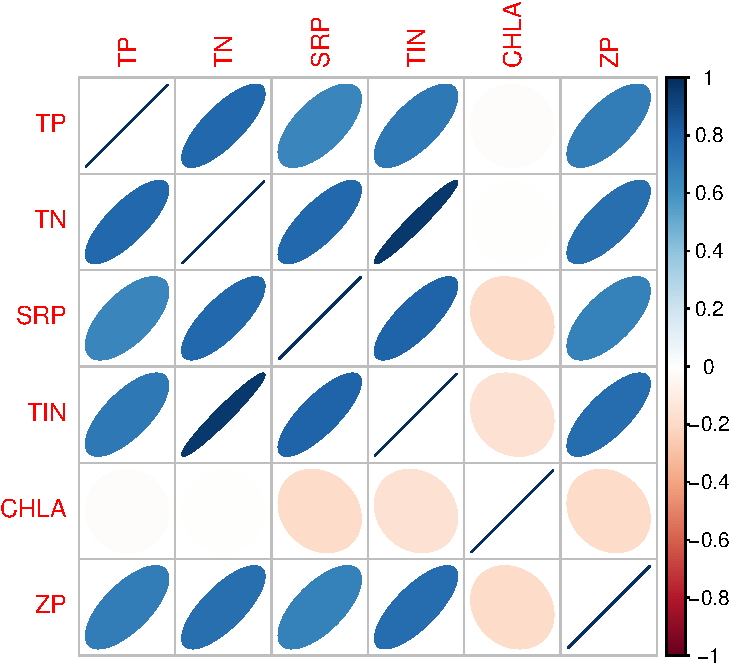
\includegraphics{5.AlphaDiversity_Worksheet_files/figure-latex/unnamed-chunk-11-1.pdf}

\textbf{\emph{Question 5}}: What effect does visualizing species
abundance data on a log-scaled axis have on how we interpret evenness in
the RAC?

\begin{quote}
\textbf{\emph{Answer 5}}: Using a log transformed y-axis helps to
compress the higher value data points and spread more evenly low data
points to make the graph more readable. If we used a linear graph, all
singletons would be overlapping and it would be difficult to distinguish
how many rare taxa there are. Using a log-scale also limits the
influence of highly abundant taxa.
\end{quote}

Now that we have visualized unevennes, it is time to quantify it using
Simpson's evenness (\(E_{1/D}\)) and Smith and Wilson's evenness index
(\(E_{var}\)).

\subsubsection{\texorpdfstring{Simpson's evenness
(\(E_{1/D}\))}{Simpson's evenness (E\_\{1/D\})}}\label{simpsons-evenness-e_1d}

In the R code chunk below, do the following:

\begin{enumerate}
\def\labelenumi{\arabic{enumi}.}
\item
  Write the function to calculate \(E_{1/D}\), and
\item
  Calculate \(E_{1/D}\) for \texttt{site1}.
\end{enumerate}

\begin{Shaded}
\begin{Highlighting}[]
\NormalTok{SimpE }\OtherTok{\textless{}{-}} \ControlFlowTok{function}\NormalTok{(}\AttributeTok{x =} \StringTok{""}\NormalTok{)\{}
\NormalTok{ S }\OtherTok{\textless{}{-}} \FunctionTok{S.obs}\NormalTok{(x)}
\NormalTok{ x }\OtherTok{=} \FunctionTok{as.data.frame}\NormalTok{(x)}
\NormalTok{ D }\OtherTok{\textless{}{-}} \FunctionTok{diversity}\NormalTok{(x, }\StringTok{"inv"}\NormalTok{)}
\NormalTok{ E }\OtherTok{\textless{}{-}}\NormalTok{ (D)}\SpecialCharTok{/}\NormalTok{S}
 \FunctionTok{return}\NormalTok{(E)}
\NormalTok{\}}

\NormalTok{site1 }\OtherTok{\textless{}{-}}\NormalTok{ BCI[}\DecValTok{1}\NormalTok{, ]}
\FunctionTok{SimpE}\NormalTok{(site1)}
\end{Highlighting}
\end{Shaded}

\begin{verbatim}
##         1 
## 0.4238232
\end{verbatim}

\subsubsection{\texorpdfstring{Smith and Wilson's evenness index
(\(E_{var}\))}{Smith and Wilson's evenness index (E\_\{var\})}}\label{smith-and-wilsons-evenness-index-e_var}

In the R code chunk below, please do the following:

\begin{enumerate}
\def\labelenumi{\arabic{enumi}.}
\item
  Write the function to calculate \(E_{var}\),
\item
  Calculate \(E_{var}\) for \texttt{site1}, and
\item
  Compare \(E_{1/D}\) and \(E_{var}\).
\end{enumerate}

\begin{Shaded}
\begin{Highlighting}[]
\NormalTok{Evar }\OtherTok{\textless{}{-}} \ControlFlowTok{function}\NormalTok{(x)\{}
\NormalTok{  x }\OtherTok{\textless{}{-}} \FunctionTok{as.vector}\NormalTok{(x[x }\SpecialCharTok{\textgreater{}} \DecValTok{0}\NormalTok{])}
  \DecValTok{1} \SpecialCharTok{{-}}\NormalTok{ (}\DecValTok{2}\SpecialCharTok{/}\NormalTok{pi) }\SpecialCharTok{*} \FunctionTok{atan}\NormalTok{(}\FunctionTok{var}\NormalTok{(}\FunctionTok{log}\NormalTok{(x)))}
\NormalTok{  \}}

\NormalTok{site1 }\OtherTok{\textless{}{-}}\NormalTok{ BCI[}\DecValTok{1}\NormalTok{, ]}
\FunctionTok{Evar}\NormalTok{(site1)}
\end{Highlighting}
\end{Shaded}

\begin{verbatim}
## [1] 0.5067211
\end{verbatim}

\textbf{\emph{Question 6}}: Compare estimates of evenness for
\texttt{site1} of BCI using \(E_{1/D}\) and \(E_{var}\). Do they agree?
If so, why? If not, why? What can you infer from the results.

\begin{quote}
\textbf{\emph{Answer 6}}: The two esimates do not agree - Evar estimates
that the species are more even than simpsons evenness estimates. Evar
log-transforms abundance data to decrease the bias introduced by heavily
abundant species. Thus, this metric is more likely a better indicator of
the true species evenness of the BCI data. We can infer that the species
evenness of the BCI dataset is moderately even.
\end{quote}

\subsection{5) INTEGRATING RICHNESS AND EVENNESS: DIVERSITY
METRICS}\label{integrating-richness-and-evenness-diversity-metrics}

So far, we have introduced two primary aspects of diversity, i.e.,
richness and evenness. Here, we will use popular indices to estimate
diversity, which explicitly incorporate richness and evenness. We will
write our own diversity functions and compare them against the functions
in \texttt{vegan}.

\subsubsection{Shannon's diversity (a.k.a., Shannon's
entropy)}\label{shannons-diversity-a.k.a.-shannons-entropy}

In the R code chunk below, please do the following:

\begin{enumerate}
\def\labelenumi{\arabic{enumi}.}
\item
  Provide the code for calculating H' (Shannon's diversity),
\item
  Compare this estimate with the output of \texttt{vegan}'s diversity
  function using method = ``shannon''.
\end{enumerate}

\begin{Shaded}
\begin{Highlighting}[]
\NormalTok{ShanH }\OtherTok{\textless{}{-}} \ControlFlowTok{function}\NormalTok{(}\AttributeTok{x =} \StringTok{""}\NormalTok{)\{}
\NormalTok{  H }\OtherTok{=} \DecValTok{0}
  \ControlFlowTok{for}\NormalTok{ (n\_i }\ControlFlowTok{in}\NormalTok{ x)\{}
    \ControlFlowTok{if}\NormalTok{ (n\_i }\SpecialCharTok{\textgreater{}} \DecValTok{0}\NormalTok{) \{}
\NormalTok{      p }\OtherTok{=}\NormalTok{ n\_i }\SpecialCharTok{/} \FunctionTok{sum}\NormalTok{(x)}
\NormalTok{      H }\OtherTok{=}\NormalTok{ H }\SpecialCharTok{{-}}\NormalTok{ p}\SpecialCharTok{*}\FunctionTok{log}\NormalTok{(p)}
\NormalTok{    \}}
\NormalTok{  \}}
  \FunctionTok{return}\NormalTok{(H)}
\NormalTok{\}}
\FunctionTok{ShanH}\NormalTok{(site1)}
\end{Highlighting}
\end{Shaded}

\begin{verbatim}
## [1] 4.018412
\end{verbatim}

\begin{Shaded}
\begin{Highlighting}[]
\FunctionTok{diversity}\NormalTok{(site1, }\AttributeTok{index =} \StringTok{"shannon"}\NormalTok{)}
\end{Highlighting}
\end{Shaded}

\begin{verbatim}
## [1] 4.018412
\end{verbatim}

\subsubsection{Simpson's diversity (or
dominance)}\label{simpsons-diversity-or-dominance}

In the R code chunk below, please do the following:

\begin{enumerate}
\def\labelenumi{\arabic{enumi}.}
\item
  Provide the code for calculating D (Simpson's diversity),
\item
  Calculate both the inverse (1/D) and 1 - D,
\item
  Compare this estimate with the output of
  \texttt{vegan\textquotesingle{}s} diversity function using method =
  ``simp''.
\end{enumerate}

\begin{Shaded}
\begin{Highlighting}[]
\NormalTok{SimpD }\OtherTok{\textless{}{-}} \ControlFlowTok{function}\NormalTok{(}\AttributeTok{x =} \StringTok{""}\NormalTok{)\{}
\NormalTok{  D }\OtherTok{=} \DecValTok{0}
\NormalTok{  N }\OtherTok{=} \FunctionTok{sum}\NormalTok{(x)}
  \ControlFlowTok{for}\NormalTok{ (n\_i }\ControlFlowTok{in}\NormalTok{ x)\{}
\NormalTok{    D }\OtherTok{=}\NormalTok{ D }\SpecialCharTok{+}\NormalTok{ (n\_i}\SpecialCharTok{\^{}}\DecValTok{2}\NormalTok{)}\SpecialCharTok{/}\NormalTok{(N}\SpecialCharTok{\^{}}\DecValTok{2}\NormalTok{)}
\NormalTok{  \}}
  \FunctionTok{return}\NormalTok{(D)}
\NormalTok{\}}

\NormalTok{D.inv }\OtherTok{\textless{}{-}}\DecValTok{1}\SpecialCharTok{/}\FunctionTok{SimpD}\NormalTok{(site1)}
\NormalTok{D.sub }\OtherTok{\textless{}{-}} \DecValTok{1}\SpecialCharTok{{-}}\FunctionTok{SimpD}\NormalTok{(site1)}
\FunctionTok{print}\NormalTok{(D.inv)}
\end{Highlighting}
\end{Shaded}

\begin{verbatim}
## [1] 39.41555
\end{verbatim}

\begin{Shaded}
\begin{Highlighting}[]
\FunctionTok{print}\NormalTok{(D.sub)}
\end{Highlighting}
\end{Shaded}

\begin{verbatim}
## [1] 0.9746293
\end{verbatim}

\begin{Shaded}
\begin{Highlighting}[]
\FunctionTok{diversity}\NormalTok{(site1, }\StringTok{"inv"}\NormalTok{)}
\end{Highlighting}
\end{Shaded}

\begin{verbatim}
## [1] 39.41555
\end{verbatim}

\begin{Shaded}
\begin{Highlighting}[]
\FunctionTok{diversity}\NormalTok{(site1, }\StringTok{"simp"}\NormalTok{)}
\end{Highlighting}
\end{Shaded}

\begin{verbatim}
## [1] 0.9746293
\end{verbatim}

\subsubsection{\texorpdfstring{Fisher's
\(\boldsymbol\alpha\)}{Fisher's \textbackslash boldsymbol\textbackslash alpha}}\label{fishers-boldsymbolalpha}

In the R code chunk below, please do the following:

\begin{enumerate}
\def\labelenumi{\arabic{enumi}.}
\item
  Provide the code for calculating Fisher's \(\boldsymbol\alpha\),
\item
  Calculate Fisher's \(\boldsymbol\alpha\) for \texttt{site1} of BCI.
\end{enumerate}

\begin{Shaded}
\begin{Highlighting}[]
\NormalTok{rac }\OtherTok{\textless{}{-}} \FunctionTok{as.vector}\NormalTok{(site1[site1 }\SpecialCharTok{\textgreater{}} \DecValTok{0}\NormalTok{])}
\NormalTok{invD }\OtherTok{\textless{}{-}} \FunctionTok{diversity}\NormalTok{(rac, }\StringTok{"inv"}\NormalTok{)}
\FunctionTok{print}\NormalTok{(invD)}
\end{Highlighting}
\end{Shaded}

\begin{verbatim}
## [1] 39.41555
\end{verbatim}

\begin{Shaded}
\begin{Highlighting}[]
\NormalTok{Fisher }\OtherTok{\textless{}{-}} \FunctionTok{fisher.alpha}\NormalTok{(rac)}
\NormalTok{Fisher}
\end{Highlighting}
\end{Shaded}

\begin{verbatim}
## [1] 35.67297
\end{verbatim}

\textbf{\emph{Question 7}}: How is Fisher's \(\boldsymbol\alpha\)
different from \(E_{H'}\) and \(E_{var}\)? What does Fisher's
\(\boldsymbol\alpha\) take into account that \(E_{H'}\) and \(E_{var}\)
do not?

\begin{quote}
\textbf{\emph{Answer 7}}: Fisher's alpha is different from Shannon's
Diversity and Smith and Wilson's Evenness index because it as the latter
two calculate diversity and evenness metrics (respectively), rather than
truly estimating their values from the given data. Fishers alpha is a
fitted parameter that estimates diversity using the rank-abunance curve.
This metric accounts for sampling errors that often occur in ecological
studies.
\end{quote}

\subsection{6) HILL NUMBERS}\label{hill-numbers}

Remember that we have learned about the advantages of Hill Numbers to
measure and compare diversity among samples. We also learned to explore
the effects of rare species in a community by examining diversity for a
series of exponents \(q\).

\textbf{\emph{Question 8}}: Using \texttt{site1} of BCI and
\texttt{vegan} package, a) calculate Hill numbers for \(q\) exponent 0,
1 and 2 (richness, exponential Shannon's entropy, and inverse Simpson's
diversity). b) Interpret the effect of rare species in your community
based on the response of diversity to increasing exponent \(q\).

\begin{quote}
\textbf{\emph{Answer 8a}}:
\end{quote}

\begin{Shaded}
\begin{Highlighting}[]
\NormalTok{q.val }\OtherTok{\textless{}{-}} \FunctionTok{tsallis}\NormalTok{(site1, }\AttributeTok{scales =} \FunctionTok{seq}\NormalTok{(}\DecValTok{0}\NormalTok{,}\DecValTok{2}\NormalTok{,}\DecValTok{1}\NormalTok{), }\AttributeTok{hill=}\ConstantTok{TRUE}\NormalTok{)}
\FunctionTok{print}\NormalTok{(q.val)}
\end{Highlighting}
\end{Shaded}

\begin{verbatim}
##        0        1        2 
## 93.00000 55.61270 39.41555 
## attr(,"class")
## [1] "tsallis" "renyi"   "numeric"
\end{verbatim}

\begin{Shaded}
\begin{Highlighting}[]
\NormalTok{hill.df }\OtherTok{\textless{}{-}} \FunctionTok{data.frame}\NormalTok{(}\AttributeTok{scale =} \FunctionTok{seq}\NormalTok{(}\DecValTok{0}\NormalTok{, }\DecValTok{2}\NormalTok{, }\DecValTok{1}\NormalTok{), }\AttributeTok{q.val =}\NormalTok{ q.val)}
\FunctionTok{plot}\NormalTok{(hill.df}\SpecialCharTok{$}\NormalTok{scale, hill.df}\SpecialCharTok{$}\NormalTok{q.val, }\AttributeTok{type =} \StringTok{"b"}\NormalTok{, }\AttributeTok{pch =} \DecValTok{19}\NormalTok{, }\AttributeTok{col =} \StringTok{"lightblue"}\NormalTok{,}
     \AttributeTok{xlab =} \StringTok{"q value"}\NormalTok{, }\AttributeTok{ylab =} \StringTok{"Diversity"}\NormalTok{)}
\end{Highlighting}
\end{Shaded}

\includegraphics{5.AlphaDiversity_Worksheet_files/figure-latex/unnamed-chunk-17-1.pdf}

\begin{quote}
\textbf{DISCLAIMER: I used copilot to help me make the graph!}
\end{quote}

\begin{quote}
\textbf{\emph{Answer 8b}}: It seems as though both abundant and rare
species are present in the community, but abudant species make up a much
larger portion of the community that the combination of rare species.
The species richness (q=0) is 93 - this value is not impacted by
abudance and thus all species are weighted equally. The impact of
abundance increases from q=1 (Shannon's Entropy) to q=2 (inverse
Simpson's diversity), and in the graph we can see a very sharp decline
in diversity as q value increases. This suggests that abundant species
make up the bulk of the community and thus negatively influence
diversity measures.
\end{quote}

\#\#7) MOVING BEYOND UNIVARIATE METRICS OF \(\alpha\) DIVERSITY

The diversity metrics that we just learned about attempt to integrate
richness and evenness into a single, univariate metric. Although useful,
information is invariably lost in this process. If we go back to the
rank-abundance curve, we can retrieve additional information -- and in
some cases -- make inferences about the processes influencing the
structure of an ecological system.

\subsection{Species abundance models}\label{species-abundance-models}

The RAC is a simple data structure that is both a vector of abundances.
It is also a row in the site-by-species matrix (minus the zeros, i.e.,
absences).

Predicting the form of the RAC is the first test that any biodiversity
theory must pass and there are no less than 20 models that have
attempted to explain the uneven form of the RAC across ecological
systems.

In the R code chunk below, please do the following:

\begin{enumerate}
\def\labelenumi{\arabic{enumi}.}
\item
  Use the \texttt{radfit()} function in the \texttt{vegan} package to
  fit the predictions of various species abundance models to the RAC of
  \texttt{site1} in BCI,
\item
  Display the results of the \texttt{radfit()} function, and
\item
  Plot the results of the \texttt{radfit()} function using the code
  provided in the handout.
\end{enumerate}

\begin{Shaded}
\begin{Highlighting}[]
\NormalTok{RACresults }\OtherTok{\textless{}{-}} \FunctionTok{radfit}\NormalTok{(site1)}
\FunctionTok{print}\NormalTok{(RACresults)}
\end{Highlighting}
\end{Shaded}

\begin{verbatim}
## 
## RAD models, family poisson 
## No. of species 93, total abundance 448
## 
##            par1      par2     par3    Deviance AIC      BIC     
## Null                                   39.5261 315.4362 315.4362
## Preemption  0.042797                   21.8939 299.8041 302.3367
## Lognormal   1.0687    1.0186           25.1528 305.0629 310.1281
## Zipf        0.11033  -0.74705          61.0465 340.9567 346.0219
## Mandelbrot  100.52   -2.312    24.084   4.2271 286.1372 293.7350
\end{verbatim}

\begin{Shaded}
\begin{Highlighting}[]
\FunctionTok{plot.new}\NormalTok{()}
\FunctionTok{plot}\NormalTok{(RACresults, }\AttributeTok{las =} \DecValTok{1}\NormalTok{, }\AttributeTok{cex.lab =} \FloatTok{1.4}\NormalTok{, }\AttributeTok{cex.axis =} \FloatTok{1.25}\NormalTok{)}
\end{Highlighting}
\end{Shaded}

\includegraphics{5.AlphaDiversity_Worksheet_files/figure-latex/unnamed-chunk-18-1.pdf}

\textbf{\emph{Question 9}}: Answer the following questions about the
rank abundance curves: a) Based on the output of \texttt{radfit()} and
plotting above, discuss which model best fits our rank-abundance curve
for \texttt{site1}? b) Can we make any inferences about the forces,
processes, and/or mechanisms influencing the structure of our system,
e.g., an ecological community?

\begin{quote}
\textbf{\emph{Answer 9a}}: Mandelbrot seems to fit our RAC best both
qualitatively as shown by the graph, as well as quantitatively as the
Mandelbrot model has the lowest AIC and BIC values. \textbf{\emph{Answer
9b}}: No, we cannot infer on any ecological influences based on this
model.
\end{quote}

\textbf{\emph{Question 10}}: Answer the following questions about the
preemption model: a. What does the preemption model assume about the
relationship between total abundance (\emph{N}) and total resources that
can be preempted? b. Why does the niche preemption model look like a
straight line in the RAD plot?

\begin{quote}
\textbf{\emph{Answer 10a}}: The model assumes a positive relationship
between the two, meaning a species with a higher abundance (N) will be
able to preempt more of the resources available. \textbf{\emph{Answer
10b}}: The niche preemption model is a straight line in the RAD plot
because when the underlying equation, a\^{}(r) = N · α · (1 −
α)\^{}(r−1), is log-transformed it becomes a variation of the linear
equation y=mx+b .
\end{quote}

\textbf{\emph{Question 10}}: Why is it important to account for the
number of parameters a model uses when judging how well it explains a
given set of data?

\begin{quote}
\textbf{\emph{Answer 11}}: Generally, its good to avoid incorporating
too many parameters because 1) the more parameters the more specific the
model is to the current dataset it is being trained on, and will most
likely result in poor fits for new data, and 2) it becomes harder to
intuit the meanings behind model results.
\end{quote}

\subsection{SYNTHESIS}\label{synthesis}

\begin{enumerate}
\def\labelenumi{\arabic{enumi}.}
\tightlist
\item
  As stated by Magurran (2004) the \({D = } \sum p_i^2\) derivation of
  Simpson's Diversity only applies to communities of infinite size. For
  anything but an infinitely large community, Simpson's Diversity index
  is calculated as \({D = } \sum \frac{n_i(n_i -1)} {N(N-1)}\). Assuming
  a finite community, calculate Simpson's D, 1 - D, and Simpson's
  inverse (i.e.~1/D) for \texttt{site\ 1} of the BCI site-by-species
  matrix.
\end{enumerate}

\begin{Shaded}
\begin{Highlighting}[]
\CommentTok{\# Simpson\textquotesingle{}s Diversity}
\NormalTok{SimpD }\OtherTok{\textless{}{-}} \ControlFlowTok{function}\NormalTok{(}\AttributeTok{x =} \StringTok{""}\NormalTok{)\{}
\NormalTok{  D }\OtherTok{=} \DecValTok{0}
\NormalTok{  N }\OtherTok{=} \FunctionTok{sum}\NormalTok{(x)}
  \ControlFlowTok{for}\NormalTok{ (n\_i }\ControlFlowTok{in}\NormalTok{ x)\{}
\NormalTok{    D }\OtherTok{=}\NormalTok{ D }\SpecialCharTok{+}\NormalTok{ (n\_i}\SpecialCharTok{\^{}}\DecValTok{2}\NormalTok{)}\SpecialCharTok{/}\NormalTok{(N}\SpecialCharTok{\^{}}\DecValTok{2}\NormalTok{)}
\NormalTok{  \}}
  \FunctionTok{return}\NormalTok{(D)}
\NormalTok{\}}

\FunctionTok{SimpD}\NormalTok{(site1)}
\end{Highlighting}
\end{Shaded}

\begin{verbatim}
## [1] 0.0253707
\end{verbatim}

\begin{Shaded}
\begin{Highlighting}[]
\NormalTok{D.inv }\OtherTok{\textless{}{-}}\DecValTok{1}\SpecialCharTok{/}\FunctionTok{SimpD}\NormalTok{(site1)}
\NormalTok{D.sub }\OtherTok{\textless{}{-}} \DecValTok{1}\SpecialCharTok{{-}}\FunctionTok{SimpD}\NormalTok{(site1)}
\FunctionTok{print}\NormalTok{(D.inv)}
\end{Highlighting}
\end{Shaded}

\begin{verbatim}
## [1] 39.41555
\end{verbatim}

\begin{Shaded}
\begin{Highlighting}[]
\FunctionTok{print}\NormalTok{(D.sub)}
\end{Highlighting}
\end{Shaded}

\begin{verbatim}
## [1] 0.9746293
\end{verbatim}

\begin{enumerate}
\def\labelenumi{\arabic{enumi}.}
\setcounter{enumi}{1}
\tightlist
\item
  Along with the rank-abundance curve (RAC), another way to visualize
  the distribution of abundance among species is with a histogram
  (a.k.a., frequency distribution) that shows the frequency of different
  abundance classes. For example, in a given sample, there may be 10
  species represented by a single individual, 8 species with two
  individuals, 4 species with three individuals, and so on. In fact, the
  rank-abundance curve and the frequency distribution are the two most
  common ways to visualize the species-abundance distribution (SAD) and
  to test species abundance models and biodiversity theories. To address
  this homework question, use the R function \textbf{hist()} to plot the
  frequency distribution for \texttt{site\ 1} of the BCI site-by-species
  matrix, and describe the general pattern you see.
\end{enumerate}

\begin{Shaded}
\begin{Highlighting}[]
\NormalTok{site1.num }\OtherTok{\textless{}{-}} \FunctionTok{as.numeric}\NormalTok{(site1)}
\FunctionTok{str}\NormalTok{(site1.num)}
\end{Highlighting}
\end{Shaded}

\begin{verbatim}
##  num [1:225] 0 0 0 0 0 0 2 0 0 0 ...
\end{verbatim}

\begin{Shaded}
\begin{Highlighting}[]
\FunctionTok{hist}\NormalTok{(site1.num, }\AttributeTok{breaks =} \FunctionTok{max}\NormalTok{(site1.num), }
     \AttributeTok{xlab =} \StringTok{"Number of Individuals"}\NormalTok{, }\AttributeTok{ylab =} \StringTok{"Frequency of Species"}\NormalTok{, }\AttributeTok{col =} \StringTok{"lightblue"}\NormalTok{, }\AttributeTok{border =} \StringTok{"black"}\NormalTok{)}
\end{Highlighting}
\end{Shaded}

\includegraphics{5.AlphaDiversity_Worksheet_files/figure-latex/unnamed-chunk-20-1.pdf}
\textgreater{} \textbf{DISCLAIMER: I used copilot to help me create the
histogram!}

\begin{enumerate}
\def\labelenumi{\arabic{enumi}.}
\setcounter{enumi}{2}
\tightlist
\item
  We asked you to find a biodiversity dataset with your partner. This
  data could be one of your own or it could be something that you
  obtained from the literature. Load that dataset. How many sites are
  there? How many species are there in the entire site-by-species
  matrix? Any other interesting observations based on what you learned
  this week?
\end{enumerate}

\begin{Shaded}
\begin{Highlighting}[]
\NormalTok{fungabundance }\OtherTok{\textless{}{-}} \FunctionTok{read.table}\NormalTok{(}\StringTok{"data/MAT\_fungal\_abundances.txt"}\NormalTok{, }\AttributeTok{sep =} \StringTok{"}\SpecialCharTok{\textbackslash{}t}\StringTok{"}\NormalTok{, }\AttributeTok{header =} \ConstantTok{TRUE}\NormalTok{) }
\NormalTok{funabun.t }\OtherTok{\textless{}{-}} \FunctionTok{as.data.frame}\NormalTok{(}\FunctionTok{t}\NormalTok{(fungabundance))}
\end{Highlighting}
\end{Shaded}

\begin{quote}
There are about 44 different species or OTUs in this dataset across 4
different sites. This dataset is interesting because it also includes
information about different treatments. The communities being assessed
are symbiotic fungal communities inside deciduous ectomycorrhizal (EcM)
shrub root tips. The root tips were exposed to different treatments:
warming, fertilizer, or warming + fertilizer.
\end{quote}

\subsection{SUBMITTING YOUR
ASSIGNMENT}\label{submitting-your-assignment}

Use Knitr to create a PDF of your completed
5.AlphaDiversity\_Worksheet.Rmd document, push it to GitHub, and create
a pull request. Please make sure your updated repo include both the pdf
and RMarkdown files.

Unless otherwise noted, this assignment is due on \textbf{Wednesday,
January 29\textsuperscript{th}, 2025 at 12:00 PM (noon)}.

\end{document}
